\subsubsection{General Trends}

% Participants were given 4 calendar weeks to complete the case studies.
% All participants are volunteers, and their participation was conducted outside of normal work or educational responsibilities.
% This 4-week optimization window factors to be $0.2\%$ of typical wind farm's 20-year lifespan \cite{HerbertAcero2014}, and we submit that optimizations (even if needing the full extent of this timeframe) would be worth the time they require, if able to produce superior results.
% However, from the participant self-reported wall-times, none of the optimizations took nearly that long.

% For this reason, we discounted required wall time as a distinguishing factor, and use resultant AEP as our only metric for measuring algorithm effectiveness.
% Though factors like processing time and computing power do vary, we consider algorithms that produce results anywhere within the 4 week announcement-to-call window to be acceptable for applications in industry.

%The participant data is multivariate, leading to numerous inferences.
As a general trend, gradient-based methods performed better in discovering a relative optima, especially for smaller farm sizes.
Some gradient-based algorithms improved in comparative AEP ranking as the number of design variables increased (\textit{sub10}, \textit{sub3}), while others degraded (\textit{sub5}, \textit{sub8}).
Simultaneously, one gradient-free algorithm increaseed in effectiveness as design variables increased (\textit{sub3}), while others competed for lowest comparative performance, regardless of farm size (\textit{sub6}, \textit{sub7}, \textit{sub9}).

Despite these multivariate results, one clear front-runner did emerge.
Regardless of wind farm size, \textit{sub4}'s algorithm consistently discovered turbine placements that delivered an AEP superior to all other participants.
A summary of \textit{sub4}'s method is included in a following section.

Also of note, as the number of design variables increased, the relative disparity between proposed optimal AEPs likewise diverged.
For the 16-turbine case, the highest result was $7.88\%$ better than the lowest.
For the 36 and 64 cases, the highest result was $11.45\%$ and $13.54\%$ better than the lowest, respectively.

% \subsubsection{AEP vs Wall Time}

% 	\cref{fig:AEPvsTime} is a plot of AEP from each submission's turbine layout, verses reported wall time for the 64 turbine case, per optimization. Note that in the call for participation, we may not have stressed enough that time and computational expense were important metrics in this study. Therefore, it is possible that many of these reported times were not measured during optimization runs and may have been estimates. 
% % 	
% 	Under the premise that these reported times are accurate, \cref{fig:AEPvsTime} shows the SNOPT\texttt{+}WEC method, though reporting the highest AEP turbine arrangement also may have taken much more time than some other approaches.

% 	More testing could be done to determine if the other methods, when permitted to run longer, would discover an optimum better than that discovered by \textit{sub4}, or if by nature of the algorithms, no matter the time limit permitted to run there are some optima unattainable by their formulations.

\subsubsection{Analysis of Best Results}

	%\subsubsubsection{Gradient-based}

	For all three farm sizes, the superior method was implemented by \textit{sub4}, using a gradient-based method.
	Coded in Python and FORTRAN, it combined SNOPT \cite{SNOPT} with a method called Wake Expansion Continuation (WEC) \cite{ThomasNing2018}.
	Running 200 optimizations, \textit{sub4} had one optimization run start from the provided example layout, and the other 199 use randomized turbine starting locations within the farm boundary.

	The WEC method is specifically designed to reduce the multimodality found in wind farm layout optimization.
	In the cited paper \cite{ThomasNing2018}, it is shown to be a method which converts design spaces with many local minima into curves approaching convexity, allowing gradient-based optimizations to more easily find the better solutions.
	An example of such ``relaxation'' to convexity is included in \cref{fig:wec1,fig:wec2}, reproduced with permission.

	\begin{figure}
		\centering
		\begin{minipage}{.43\textwidth}
		  \centering
		  \captionsetup{width=0.77\textwidth}
		  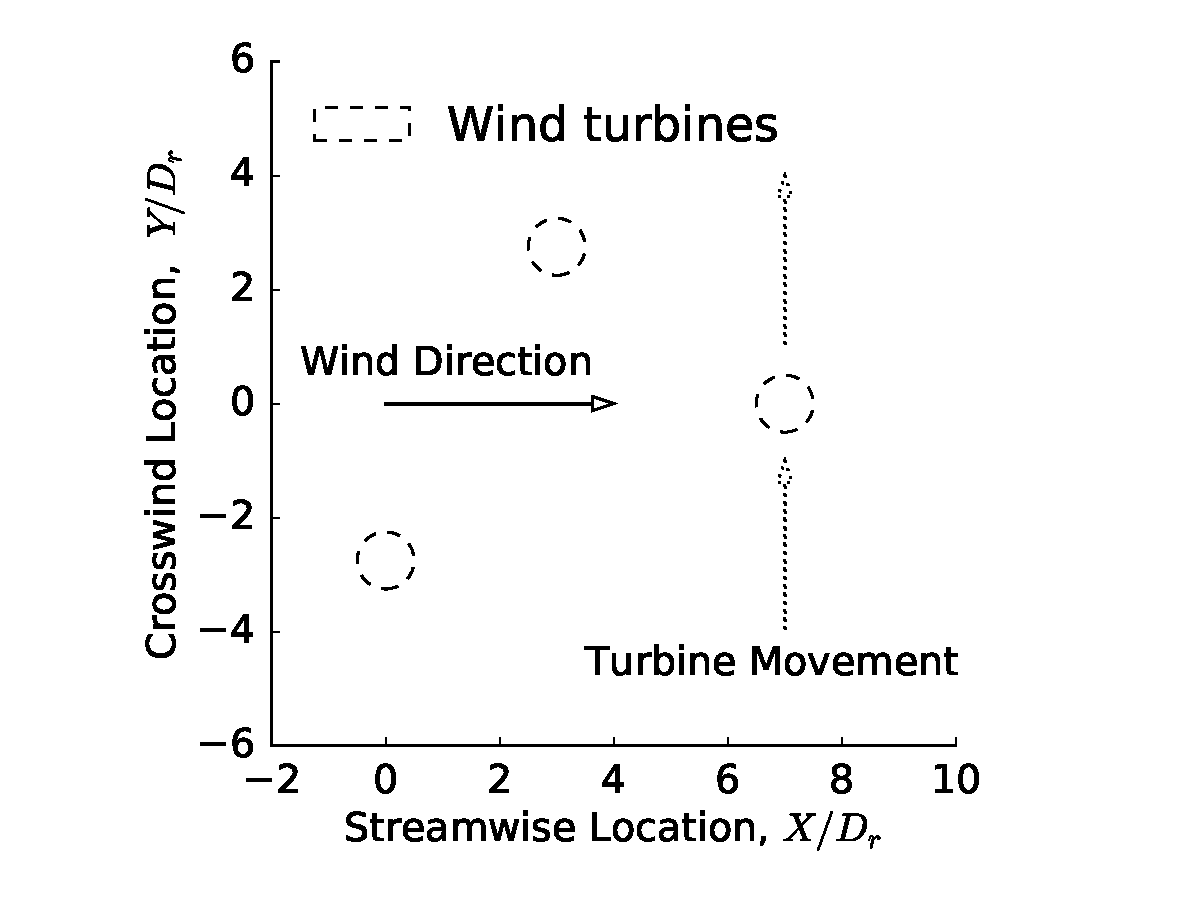
\includegraphics[width=\textwidth]{./figures/thomas-wec1.pdf}
		  \caption{Simple design space used to
		  	demonstrate the effects of the relaxation
			factor, $\xi$, on the wind farm layout design space. \cite{ThomasNing2018}}
		  \label{fig:wec1}
		\end{minipage}%
		\begin{minipage}{.5\textwidth}
		  \centering
		  \captionsetup{width=0.94\textwidth}
		  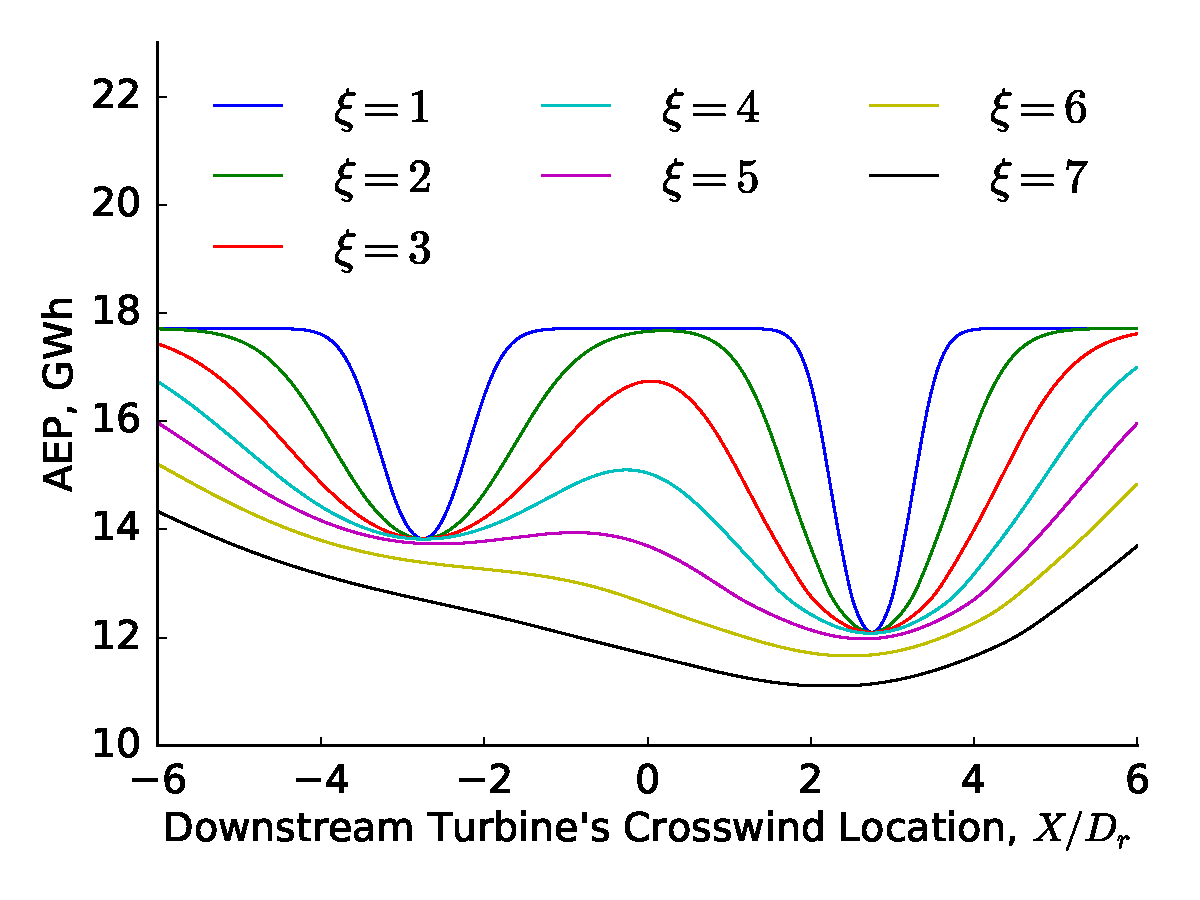
\includegraphics[width=\textwidth]{./figures/thomas-wec2.pdf}
		  \caption{The impact of the wake relaxation factor, $\xi$.
		  One turbine was moved across the wakes of two upstream turbines (see \cref{fig:wec1}). \cite{ThomasNing2018}}
		  \label{fig:wec2}
		\end{minipage}
	\end{figure}

	The effect of the WEC method on a simple design space is shown in \cref{fig:wec1,fig:wec2}. WEC smooths out the local optima, making better solutions available to gradient-based optimization methods. As the authors Thomas and Ning state, ``Larger values of $\xi$ allow the smaller local optima to disappear completely.
	Smaller values of $\xi$ allow for more accurate wake widths but with an increase in the number and magnitude of local optima.'' \cite{ThomasNing2018}.
	We suspect that the WEC method for reducing the multimodality of the design space is why \textit{sub4}'s optimizations found superior layouts as compared with the other methods used.

	%\subsubsubsection{Gradient-free}

	%Of the gradient-free methods used, the superior particiant was \textit{sub2}.
	%Futhermore, the relative performance increased as wind farm size increased.
	%Out of the 10 participants, \textit{sub2} ranked 5th, 3rd, then 2nd as the turbine sizes went from 16, to 36, to 64.
	
	%Programmed in Python, \textit{sub2} used a ``Preconditioned'' Sequential Quadratic Programming (SQP) optimization method.
	%SQP is an optimization method which breaks the problem into quadratic subproblems.
	%To seed steps between generations, \textit{sub2} took a starting layout and rotated it in $\pi$/6 steps.
	%The best of the 12 resultant layouts was then taken as the warm-start for the next generation.

	%still don't know how he did it. pyOpt??


% \subsubsection{Analysis of Worst Results}
% 	\subsubsubsection{Gradient-based}
	
% 	The worst performing gradient-based approach was different for each wind farm size.
% 	For the 16 turbine farm, \textit{sub10}'s method was the poorest performing gradient-based method, but climed to the second best gradient method for the large sizes.
% 	For the 36 turbine farm, \textit{sub1} was the poorest gradient-based method, but for the 64 turbine case, outperformed two other gradient-based methods.
% 	For the 36 turbine farm, \textit{sub5}'s attempt was the worst gradient-based method performance, and poorer than almost all of the gradient-free methods as well.

% 	Not using the Python implementation we supplied, \textit{sub5} translated the target AEP function into MATLAB and used that language's built-in FMINCON() function to optimize turbine locations.
% 	For the 16 farm case, \textit{sub5} did 1000 optimizations, each with randomized turbine starting locations.
% 	Due to computational time required, \textit{sub5} did only 500 random starts for the 64 turbine case, and this poorer relative performance may be a result of the smaller sample size.

% 	\subsubsubsection{Gradient-free}

% 	Two participants using gradient-free methods (\textit{sub6}, \textit{sub7}) rotated positions for lowest relative AEP.
% 	They each used a different method, and will be described individually.

% 	Coding in MATLAB, \textit{sub6} used a multi-start partical swarm, with the interior point method.
% 	For each farm size \textit{sub6} did 300 optimizations, with 20 swarm particles.
% 	If the minimum distance between turbines was violated at the end of an iteration, \textit{sub6}'s algorithm randomized a new turbine location within the boundary and spacing constraints.
% 	The swarm algorithm used an inertia weight 0.729, and social and cognitive weights of 1.49618.
% 	The initial turbine location population used only turbine coordinates satisfying the boundary and spacing constraints.

% 	Coding in Python, \textit{sub7} used a genetic algorithm.
% 	The algorithm used a tournament selection method, with n=10 and elitism, where only the highest AEP layouts went on to seed the next generation.
% 	There were 25 generations each of size 500, using a mutation probability of 3\%.

\subsubsection{Discussion}

	%For the 3 farm sizes we tested, \textit{sub4}'s strategy of using the SNOPT optimizer combined with the WEC relaxation method consistently delivered superior layouts.

	Though \textit{sub4} consistently found the superior AEP relative to the other participants, \textit{sub2}'s results demonstrated a trend closing the gap as the number of design variables increased.
	For the 16 turbine case, \textit{sub4} was 2.5\% better than \textit{sub2}'s results.
	For the 36 and 64 cases, \textit{sub4} was 1.68\% and 0.46\% better, respectively.
	It should be noted, however, that at the current average U.S. rate \cite{ChooseEnergyCost} of roughly \$0.13 for a kWh (or \$133 per MWh), the income difference between the AEPs of \textit{sub4} and \textit{sub2} in the 64 turbine case, though only 0.46\%, equates to a difference of a little under \$1 million per year.
	Since \textit{sub2}'s Preconditioned Sequential Programming (PSQP) method steadily closed the gap, a future study should test even larger wind farm sizes.
	This could determine if the PSQP algorithm could eventually outperform the SNOPT\texttt{+}WEC method when a certain number of design variables are reached, or if there is an upper limit or convergence to this trend.

	Though the majority of participants used random starts for each optimizaiton, \textit{sub2}'s method of ``warm starting'' performed progressively well, especially as the number of design variables increased.
	Taking a starting set of turbine coordinates, \textit{sub2} rotated the layout in $\pi$/6 steps.
	These rotations created the starting geometry for subsequent iterations.
	Though not precisely ``intuitive'' starts, they are more intelligently designed than pure randomized locations.
	As discussed above, \textit{sub2} did perform increasingly well compared to other methods (ranking 2nd for the 64-turbine case).
% 	But more importantly, as can be seen in \cref{fig:AEPvsTime}, \textit{sub2} while getting within $0.46 \%$ from the best solution, took less average time per iteration by an order of magnitude.
% 	So while the ``warm start'' rotation method wasn't able to find an AEP superior to \textit{sub4}, it reached an optimized solution much more quickly.
	
	Translating the provided AEP target function proved helpful in speeding up the computations and allowing for greater exploration.
	At least two participants translated the target Python file into FORTRAN, one into Julia, and one altered it within Python by converting loops into vectorized statements.
	In testing, these reimplementations sped up the analysis time by at least an order of magnitude. 
	
	In our survey we asked participants to self-report time and iteration count for their optimizations.  However, the question was not clearly worded resulting in different interpretations.  Some reported the time for their best optimization run, while others included total time include exploratory runs, multistarts, or other iterative approaches (the latter was intended).  Also, because we did not warn users that this information would be requested in the survey, some of the numbers were not recorded during optimization and were simply estimated.  As an example, self-reported optimization time for the 64 turbine case is shown in \cref{fig:AEPvTime} labeled by submission number.  Given the limitations in reporting described above, no real conclusions can be drawn at this time, but the data is provided to give a general sense of the algorithmic times.
	